\documentclass[11pt]{article}
\usepackage[paper=a4paper,dvips,top=2.5cm,left=2.5cm,right=2.5cm,
    foot=2cm,bottom=2.5cm]{geometry}
\usepackage[utf8]{inputenc}
\usepackage{lipsum}
\usepackage{graphicx}

\begin{document}
\setlipsumdefault{1-10}
%%%%%%%%%%%%%%%%%%%%%%%%%%%%%%%%%%%%%%%%%%%%%%%%%%%%%%%%%%%%%%%
%%%%%%%%%%%%%%%%%%%%%REMERCIEMENTS
%%%%%%%%%%%%%%%%%%%%%%%%%%%%%%%%%%%%%%%%%%%%%%%%%%%%%%%%%%%%%%%
\part*{Remerciement}
Je remercie....
\pagebreak
%%%%%%%%%%%%%%%%%%%%%%%%%%%%%%%%%%%%%%%%%%%%%%%%%%%%%%%%%%%%%%%
%%%%%%%%%%%%%%%%%%%%%ENTREPRISE
%%%%%%%%%%%%%%%%%%%%%%%%%%%%%%%%%%%%%%%%%%%%%%%%%%%%%%%%%%%%%%%
\part*{Entreprise}
Thales...
\pagebreak
%%%%%%%%%%%%%%%%%%%%%%%%%%%%%%%%%%%%%%%%%%%%%%%%%%%%%%%%%%%%%%%
%%%%%%%%%%%%%%%%%%%%%INTRO
%%%%%%%%%%%%%%%%%%%%%%%%%%%%%%%%%%%%%%%%%%%%%%%%%%%%%%%%%%%%%%%
\part*{Introduction}
Contexte
-au sein de l'entreprise
-au sein de l'equipe
-au sein du domaine technique
But du stage
-resultats attendus
-precedents resultats dans le domaine
\pagebreak
\part*{Deroulement}
\section{Contrôle caméra et flux vidéo}


Lorem ipsum dolor sit amet, consectetur adipiscing elit. Nulla non ultrices quam, et bibendum ligula. Nullam scelerisque nisi at lacus congue, at ullamcorper arcu cursus. Mauris quis viverra lacus. Morbi egestas eros id viverra volutpat. Fusce consectetur, turpis egestas aliquet cursus, turpis magna elementum urna, vel commodo leo nulla pretium lectus. Duis mattis, est et blandit tempus, lectus orci elementum mauris, sed imperdiet nulla dolor eget lacus. Fusce venenatis elit risus, quis congue risus vestibulum eu. Pellentesque sed lorem nunc. Phasellus lectus dui, consequat ac augue non, congue lobortis libero. Vivamus euismod sagittis nunc vel laoreet. Donec tortor augue, laoreet a elit at, tempus rutrum elit. Phasellus sagittis, nisi sed semper pulvinar, libero lorem facilisis urna, sit amet accumsan sapien nibh vel massa. Mauris eleifend in sapien id sagittis. Morbi luctus quam id tellus sodales, ac luctus magna sodales. Aenean sed nisi ac sapien consectetur aliquam. Sed nec ex non mi molestie euismod ut eget augue.

Donec sit amet elit accumsan, semper ante sed, laoreet metus. Proin dictum consequat sem. Nulla turpis nunc, laoreet ut tellus vitae, pulvinar mollis augue. Praesent ut quam sit amet ex ornare cursus. Quisque massa libero, hendrerit sit amet bibendum at, congue vel mi. Pellentesque libero arcu, posuere et dolor sit amet, vulputate sollicitudin orci. Mauris mollis urna a lacus posuere, non mattis nibh volutpat. Nam varius leo nulla, sit amet ullamcorper nisi sagittis ac. Nam at placerat sem, sit amet feugiat magna. Phasellus fringilla, arcu sit amet laoreet hendrerit, enim mauris iaculis tellus, pharetra gravida ipsum sem vel odio. Cum sociis natoque penatibus et magnis dis parturient montes, nascetur ridiculus mus. Donec faucibus ex ipsum, pellentesque rutrum est sollicitudin at.

Aenean sodales congue augue, vel bibendum enim interdum nec. Ut ultricies faucibus purus, et condimentum ligula ornare dictum. Aenean ornare ante eu ante dignissim congue. Etiam fringilla augue urna, ultricies vulputate arcu aliquam eu. Donec tempor commodo mi, eu accumsan elit suscipit at. Nulla sed nibh id lectus ullamcorper laoreet. Integer consequat feugiat lorem a mollis. Nulla id vulputate risus, ut aliquet dolor. Donec erat lacus, fermentum ac mi et, elementum scelerisque ex. Aliquam mauris purus, mattis sed feugiat sed, fringilla tempor enim. Sed finibus justo arcu, a ultricies mauris posuere quis. Praesent tortor justo, congue eu iaculis consequat, consectetur vitae ipsum.

Aliquam vestibulum, sapien ut maximus blandit, mi purus aliquet odio, non convallis nibh magna et quam. Nunc tincidunt tempus libero, id feugiat quam dapibus eget. Donec vitae dui a mi posuere ornare. Nunc a egestas mauris. Pellentesque iaculis neque mauris, nec malesuada lectus ullamcorper ut. Mauris quis sollicitudin sapien, euismod condimentum magna. Nunc scelerisque sagittis metus vitae posuere. Donec est urna, scelerisque aliquet metus quis, consectetur tempus dolor. Cras pharetra hendrerit congue. Nullam eget velit nisl. Aliquam erat volutpat. Etiam justo lorem, dignissim sit amet tortor at, cursus blandit lectus. Donec ut eleifend risus, eu tempor est. Etiam tincidunt felis quis mi suscipit dignissim. Donec gravida vitae libero at posuere. Ut congue odio quis rhoncus vulputate.

Quisque interdum dui suscipit tristique blandit. Cras pharetra dolor non leo porta, id accumsan libero posuere. Quisque id ante non arcu mollis viverra nec vitae ipsum. Maecenas eros metus, tristique ac augue quis, volutpat aliquet massa. Proin eget elit tortor. Mauris dignissim eros leo, sed iaculis sem tempor ut. Suspendisse cursus sapien quam, ut congue odio ultricies facilisis. Curabitur ac tristique libero.
\pagebreak
\section{Détection de personne}
Afin de mettre en place un suivi efficace des personnes, il faut commencer par être capable de détecter ces personnes. Il a donc fallu en premier lieu décider d'une méthode de detection de personnes adaptée à notre application. De nombreuses méthodes différentes existent dans ce domaine, mais l'environnement dans lequel nous effectuons cette detection fixe nos besoins:

-le suivi des personnes devant être fait en temps réel, il nous faut un algorithme suffisament rapide pour ne pas avoir un impact trop important sur les performances du système complet;

-le fait que nous travaillons avec un caméra PTZ et que ce travail soit destiné à fonctionner dans des environnements variés élimine les méthodes de detection se basant sur un fond connu.\\
\\
Mon choix s'est porté sur une détection basée sur les histogramme de gradient orienté (HOG) pour son efficacité reconnue, sa rapidité et le fait que cet algorithme est suffisament populaire pour pouvoir trouver des implementations simples et des classifieurs entrainés sur des jeu de données correspondants à notre cas de figure.
L'implementation utilisée est celle présente dans OpenCV sous le nom de 'HOGDescriptor' associé à un classifieur de type machines à vecteurs de support (SVM). Le descripteur utilisé est celui par défaut d'OpenCV pour les personnes.
\subsection{Principe de la détection HOG}
Cette méthode a été présentée par Navneet Dalal et Bill Triggs en 2005 dans le papier 'Histograms of Oriented Gradients for Human Detection'.
Elle consiste en une série d'étapes illustrées dans la figure~\ref{fig:hog_topo}.
\begin{figure}[!h]
    \label{fig:hog_topo}
    \centering
	    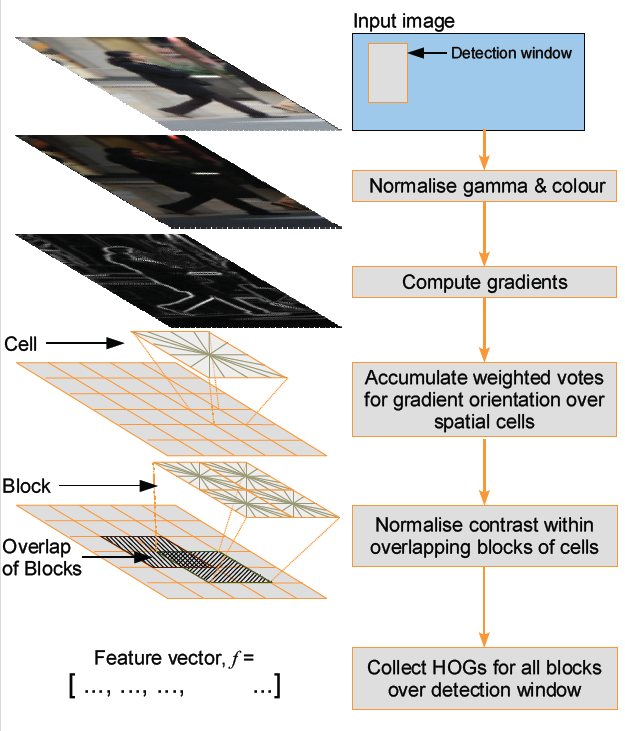
\includegraphics[width=0.7\textwidth]{hog_topo.png}
	    \caption{Illustration HOG+SVM}
\end{figure}

\subsection{SVM}
type de classifieur... machine learning toussa toussa

\subsection{Paramètres et traitement des rectangles}
-paramètres utilisés et pourquoi
-gestion des rectangles multiples

\subsection{Resultat obtenues}
-10FPS
-pratiquement aucun faux positifs
(géré par le tracking sisi)
-pratiquement complet niveau detection face/dos
(géré aussi maggle)
-lacune: detection de profil

\section{Suivi de personnes}
\section{Decision de flight plan de caméra}
\section{Detection de visage}
\pagebreak
\part*{Resultats et amélioration}
\pagebreak
\part*{Conclusion}
\pagebreak

\end{document}